\section{مروری بر روش‌های تشخیص انجمن}
ساختار انجمن‌های یک شبکه یکی از مهمترین ویژگی‌‌های ساختاری آن شبکه است. به عنوان یک تعریف کیفی، می‌توان گفت که انجمن‌ها زیرمجموعه‌هایی از گره‌های یک شبکه هستند که ارتباطات در درون آن‌ها به نسبت بیرون، بیشتر و در اصطلاح چگال‌تر است \cite{porter2009communities}. در تعریف دیگری، انجمن‌ها گروهی از گره‌ها خوانده می‌شوند که احتمالاً ویژگی‌های مشترک دارند و یا نقش‌های مشابهی در شبکه ایفا می‌کنند \cite{fortunato2010community}. برای مثال در یک شبکهٔ اجتماعی، دانشجویان هم‌رشته در یک دانشگاه و در مقاطع نزدیک، ارتباطات بیشتری با هم دارند و در واقع تشکیل یک انجمن می‌دهند. همین امر باعث می‌شود که اعضای یک انجمن ویژگی‌های شبیه به هم داشته باشند و علایق و سلایق آن‌ها به هم نزدیک باشد و رفتارهای مشابهی از خود نشان دهند. همچنین تاثیرگذاری اعضای یک انجمن روی بقیهٔ اعضای آن انجمن بیشتر است. مطالعهٔ انجمن‌ها به دلایل متعددی اهمیت دارد. برای مثال می‌توان از مطالعهٔ انجمن‌های یک شبکه اجتماعی، افرادی با سلیقه مشترک را شناسایی کرد و با استفاده از این کار، اهداف اجتماعی، سیاسی، تجاری و… خود را دنبال کرد.

در شکل \ref{fig:comm} می‌توان یک گراف ساده با سه انجمن را مشاهده کرد که با خط‌چین از هم جدا شده‌اند. همان‌طور که در این شکل نیز مشخص است، تعداد چگالی یال‌های درون انجمن‌ها بیشتر از بیرون آن‌هاست و گره‌ها درون انجمن‌ها روابط نزدیک‌تری به هم دارند.
\begin{figure}[!hbt]
  \begin{center}
    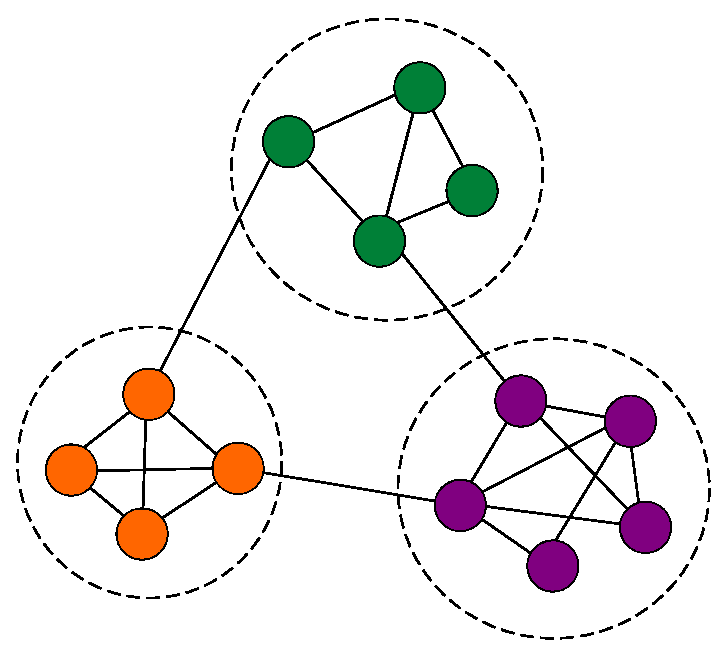
\includegraphics[width=8cm]{comm.eps}
    \caption{یک شبکهٔ نمونه با سه انجمن}
    \label{fig:comm}
  \end{center}
\end{figure}

در این بخش، ابتدا مروری خواهد شد بر روش‌های تشخیص انجمن و دسته‌بندی از آن‌ها رائه خواهد شد. سپس روش تشخیص انجمن مد نظر این پژوهش یعنی الگوریتم نقشه‌اطلاعات\LTRfootnote{Infomap} با جزییات بیشتری بررسی خواهد شد.

\subsection{انواع روش‌های تشخیص انجمن}
روش‌های تشخیص انجمن به دسته‌های مختلفی طبقه‌بندی می‌شوند و طبقه‌بندی‌های مختلفی توسط پژوهشگران مختلف از این الگوریتم‌ها ارائه شده‌است \cite{porter2009communities} \cite{fortunato2010community} \cite{yang2010discovering}. در این بخش به مرور تعدادی از این روش‌ها می‌پردازیم.

\subsubsection{روش‌های سنتی}
این روش‌ها خود به چند دسته تقسیم‌بندی می‌شوند:
\begin{description}
  \item[روش‌های افراز گراف]\LTRfootnote{Graph Partitioning}\textbf{:}
  این روش‌ها سعی می‌کنند یک گراف را به تعداد مشخصی زیرگروه با سایز مشخص تقسیم کنند، به طوری که تعداد یال‌هایی که بین زیرگروه‌ها قرار می‌گیرند کمینه باشد. به تعداد یال‌هایی که بین زیرگروه‌ها قرار می‌گیرند \textit{اندازهٔ برش}\LTRfootnote{cut size} گفته می‌شود. در این روش‌ها تعداد زیرگروه‌ها اهمیت دارد، چون اگه این پارامتر آزاد باشد، در نهایت به یک پاسخ بدیهی خواهیم رسید که همهٔ گره‌ها در یک زیرگروه قرار بگیرند. همچنین اندازهٔ زیرگروه‌ها نیز مهم است چون در صورت آزاد بودن این پارامتر نیز به یک پاسخ بدیهی دیگر خواهیم رسید که گرهی با کمترین درجه به عنوان یک زیرگروه و سایر گره‌ها به عنوان زیرگروه دیگر معرفی شوند.
  \item[روش‌های خوشه‌بندی سلسله‌مراتبی]\LTRfootnote{Heirarchical Clustering}\textbf{:}
  چون در حالت کلی اطلاعات بسیار کمی دربارهٔ تعداد خوشه‌های یک گراف وجود دارد، تعیین تعداد و اندازهٔ زیرگروه‌ها کار ساده‌ای نیست. از طرف دیگر گراف‌ها معمولن ساختاری سلسله‌مراتبی\LTRfootnote{Heirarchical} دارند به این معنی که سطح‌های مختلفی از گروه‌بندی را شامل می‌شوند و انجمن‌های کوچکتر در داخل انجمن‌های بزرگ‌تر قرار می‌گیرند. نقطه شروع این روش‌ها تعیین یک معیار شباهت بین گره‌هاست. وقتی این معیار شباهت انتخاب شد، برای هر جفت گره محاسبه می‌شود (صرف نظر از این که گره‌ها به هم متصل هستند یا نه)  و در نهایت، هدف، رسیدن به خوشه‌بندی‌ایست که شباهت داخل گروه‌ها را بیشینه کند. خود این روش‌هابه دو دسته تقسیم می‌شوند:
  \begin{enumerate}
    \item \textbf{الگوریتم‌های تجمیعی}\LTRfootnote{Agglomerative}
    که رویکردی پایین به بالا\LTRfootnote{bottom-up} دارند. در ابتدا هر گره به تنهایی یک خوشه را تشکیل می‌دهد و سپس خوشه‌هایی با بیشترین شباهت با هم ترکیب شده و خوشه‌های بزرگتر را می‌سازند و این کار تا وقتی ادامه پیدا می‌کند که یک خوشه که همهٔ گره‌ها را در بر دارد بماند.
    \item \textbf{الگوریتم‌های تقسیمی}\LTRfootnote{Divisive}
    که رویکردی بالا به پایین\LTRfootnote{top-down} دارند. در ابتدا کل گره‌های گراف یک خوشه را تشکیل می‌دهند و در ادامه این خوشه به صورت تکراری از روی یال‌هایی که کمترین شباهت را دارند شکسته می‌شوند تا در نهایت هر گره در یک خوشه قرار گیرد.
  \end{enumerate}
  از مشکلات این روش‌ها می‌توان به هزینهٔ محاسباتی بالا، وابستگی زیاد به معیار شباهت انتخاب شده، کارایی نه چندان خوب در گراف‌هایی بدون ساختار سلسله‌مراتبی، و… اشاره کرد.
  \item[روش‌های خوشه‌بندی افرازی]\LTRfootnote{Partitional clustering}\textbf{:}
  این روش‌ها نیز همان‌طور که از اسمشان پیداست، سعی می‌کنند که مجموعه داده‌ها را که همان گره‌های گراف است خوشه‌بندی کنند. در این‌جا نیز تعداد خوشه‌ها از قبل مشخص است. همچنین می‌بایست گره‌های گراف را به فضایی برد که در آن قابلیت اندازه‌گیری وجود داشته باشد و بتوان فاصلهٔ بین گره‌ها را محاسبه کرد. سپس روش‌هایی مانند \lr{$k$-means} و سایر روش‌های این خانواده را روی آن‌ها اعمال کرد.
  \item[روش‌های خوشه‌بندی طیفی]\LTRfootnote{Spectral Clustering}\textbf{:}
  در این دسته از روش‌ها نیاز است که یک ماتریس فاصله (مثل $S$) متناظر با گراف تولید شود که برای هر جفت از گره‌ها، فاصلهٔ آن‌ها را مشخص می‌کند. سپس از روش‌هایی کمک گرفته می‌شود که این ماتریس را با استفاده از بردارویژهٔ ماتریس $S$ (یا دیگر ماتریس‌هایی که با استفاده از آن به دست می‌آیند)، به خوشه‌هایی افزار کند.
\end{description}

\subsubsection{روش‌های بر پایهٔ پیمانگی}
یک روش تشخیص انجمن خوب روشی‌است که افراز خوبی انجام دهد. اما برای تعریف یک افراز خوب نیاز به یک معیار کمی داریم. یکی از مشهورترین این معیارها، \textit{پیمانگی}\LTRfootnote{Modularity} است. این معیار توسط نیومن\LTRfootnote{Newman} و گیروَن\LTRfootnote{Girvan} در سال ۲۰۰۴ معرفی شد\cite{newman2004finding}. این معیار بر پایهٔ این ایده بنا شده‌است که از یک گراف تصادفی انتظار نمی‌رود که ساختار خوشه‌ای مشخصی داشته باشد. در نتیجه می‌توان با مقایسهٔ چگالی یال‌های زیرگراف‌های به دست آمده با زیرگراف‌های یک گراف تصادفی با توزیع درجات یکسان، وجود ساختار خوشه‌ها در گراف را مشخص کرد. رابطهٔ ارائه شده برای محاسبهٔ این معیار به صورت زیر است:
\begin{equation}\label{eq:modularity}
  Q = \frac{1}{2m}\sum_{ij}{(A_{ij} - P_{ij})\delta(C_i,C_j)}
\end{equation}
که در آن مجموع، روی تمام جفت گره‌ها اعمال می‌شود. در رابطهٔ \ref{eq:modularity}، $A$ ماتریس مجاورت، $m$ تعداد کل یال‌ها و $P_{ij}$ احتمال وجود یال بین دو گرهٔ $i$ و $j$ است. تابع $\delta(i,j)$ نیز مشخص می‌کند که آیا دو گره $i$ و $j$ در یک انجمن هستند یا خیر، به این صورت که اگر عضو یک انجمن بودند مقدار $1$ و در غیر این صورت مقدار $0$ به خود می‌گیرد. در نهایت مقدار $Q$ عددی بین $+1$ و $-1$ خواهد شد که هر چه بزرگتر بودن آن نشان‌دهندهٔ بهتر بودن خوشه‌بندی خواهد بود.

در این دسته از روش‌ها، هدف بیشینه کردن مقدار $Q$ است. در نتیجه این روش‌ها، مسئلهٔ تشخیص انجمن را تبدیل به یک مسئلهٔ بهینه سازی می‌کنند. حل این مسائل بهینه‌سازی از روش‌های مختلفی مثل روش حریصانه\LTRfootnote{greedy}، روش تبرید شبیه‌سازی‌شده\LTRfootnote{simulated annealing} و غیره قابل حل است. از مشکلات این دسته روش‌ها می‌توان به افزایش سریع فضای مسئلهٔ بهینه‌سازی اشاره کرد که این روش‌ها را برای گراف‌های بزرگ نامناسب می‌کند.

\subsubsection{سایر روش‌ها}
دسته‌هایی دیگر از روش‌ها نیز مانند روش‌های استنتاج آماری\LTRfootnote{statistical inference}، الگوریتم‌های پویا\LTRfootnote{\lr{dynamic algorithms}} و… وجود دارند که توضیح آنها از حوصلهٔ این پژوهش خارج است. اما روشی که در این پژوهش مد نظر است، الگوریتم نقشه‌اطلاعات است که در دستهٔ روش‌های پویا دسته‌بندی می‌شود. در بخش بعد به توضیح در مورد این الگوریتم می‌پردازیم.

\subsection{الگوریتم نقشه‌اطلاعات}
این الگوریتم در سال ۲۰۰۸ توسط روسوَل\LTRfootnote{Rosvall} و برگستروم\LTRfootnote{Bergestrom} \cite{rosvall2008maps} به عنوان روشی برای تشخیص انجمن‌ها معرفی شد. همان‌طور که اشاره شد، این روش یک روش پویاست. در این روش سعی می‌شود که اطلاعات یک فرآیند پویا که روی یک گراف در حال شکل‌گیری است، طوری کد شود که به بهترین شکل فشرده شود. این فرآیند پویا یک ولگشت با طول بی‌نهایت است. در واقع این مسئله با بهینه‌سازی یک تابع هزینه به نام \textit{حداقل طول توصیف}\LTRfootnote{Minimim Description Length} به دست می‌آید\cite{grunwald2005advances}. این بهینه‌سازی با ترکیبی از جستجوی حریصانه و تبرید شبیه‌سازی‌شده قابل حل است.

\begin{figure}
  \begin{subfigure}{.5\textwidth}
    \centering
    \includegraphics[width=7cm]{infomap1.png}
    \caption{}
    \label{fig:infomap_a}
  \end{subfigure}
  \begin{subfigure}{.5\textwidth}
    \centering
    \includegraphics[width=7cm]{infomap2.png}
    \caption{}
    \label{fig:infomap_b}
  \end{subfigure}
  \begin{subfigure}{.5\textwidth}
    \centering
    \includegraphics[width=7cm]{infomap3.png}
    \caption{}
    \label{fig:infomap_c}
  \end{subfigure}
  \begin{subfigure}{.5\textwidth}
    \centering
    \includegraphics[width=7cm]{infomap4.png}
    \caption{}
    \label{fig:infomap_d}
  \end{subfigure}
  \caption{چگونگی عملکرد الگوریتم نقشه‌اطلاعات}
  \begin{center}
  (تصاویر برگرفته  از \cite{rosvall2010map})
  \end{center}
  \label{fig:infomap}
\end{figure}

برای روشن‌تر شدن موضوع فرض کنید می‌خواهیم ولگشت تصویر شده در شکل \ref{fig:infomap_a} را کد کنیم. کدگذاری هافمن\LTRfootnote{Huffman Coding} می‌تواند این کار را برای ما انجام دهد. با استفاده از این روش، همان‌طور که در شکل \ref{fig:infomap_b} به هر کدام از گره‌ها یک دنباله یکتا از ۰ و ۱ نسبت می‌دهیم، سپس برای کد کردن مسیر، شمارهٔ گره‌های دیده‌شده در مسیر را به ترتیب پشت سر هم قرار می‌دهیم. طول کد به دست آمده برای این مسیر ۳۱۴ بیت خواهد بود. اما یک روش دیگر برای کدگذاری این است که از یک کدگذاری دوسطحی استفاده کنیم، به این صورت که به هر کدام از خوشه‌های اصلی گراف یک کد یکتا اختصاص بدهیم، اما کد گره‌ها داخل خوشه‌ها می‌تواند مجدداً استفاده شود. این کدها در شکل‌های \ref{fig:infomap_c} و \ref{fig:infomap_d} قابل مشاهده هستند. همچنین کدهای ورود و خروج از هر خوشه نیز در شکل \ref{fig:infomap_c} به ترتیب قبل و بعد از فلش‌ها نوشته شده‌اند. با استفاده از این کدهای جدید، می‌توانیم مسیر مورد نظر را با استفاده از ۲۴۳ بیت کد کنیم. این مسیر در پایین شکل \ref{fig:infomap_c} نمایش داده شده‌است. همان‌طور که مشاهده می‌شود، با استفاده از این کدگذاری جدید توانستیم ۳۲٪ از طول کد نهایی بکاهیم.

اما این کدگذاری را می‌بایست به دست آوریم. برای این کار فرض کنید یک افراز مثل $\textsf{M}$ داریم که $n$ گره
$\alpha = 1,\ldots,n$
را به $m$ زیرمجموعه
$i = 1,\ldots,m$
افراز می‌کند. حد پایین طول کد به دست آمده توسط $\textsf{M}$ را به شکل تابع $L(\textsf{M})$ با توجه به نظریهٔ شانون تعریف می‌کنیم. تابع مورد نظر به شکل زیر تعریف می‌شود:
% \begin{equation}
%     L(\textsf{M}) = q_\curvearrowright H(\mathcal{Q}) + \sum_{i=1}^{m}{p^i_\circlearrowright H(\mathcal{P}^i)}
% \end{equation}
%این معادله توازنی میان دو عبارت برقرار می‌کند: عبارت اول که بی‌نظمی\LTRfootnote{entropy} حرکت بین خوشه‌هاست و عبارت دوم که بی‌نظمی حرکت بین خوشه‌هاست. هر کدام از این عبارات نیز وزنی متناسب با احتمال رخدادشان در افراز مورد نظر گرفته‌اند. در اینجا $q_\curvearrowright$ احتمال این است که در هر مرحله ولگشت مورد نظر خوشهٔ فعلی را ترک کند. عبارت $H(\mathcal{Q})$ بی‌نظمی کد خوشه‌ها (یعنی اعدادی که در شکل \ref{fig:infomap_d} زیر آنها خط کشیده شده) و عبارت $H(\mathcal{P}^i)$ بی‌نظمی کدِ گره‌های درون خوشهٔ $i$ (به همراه کدهای خروج از خوشه) هستند. وزن $p^i_\circlearrowright$ نیز مجموع احتمال حرکت بین گره‌های خوشهٔ $i$ به همراه احتمال خروج از خوشه $i$ است. در نهایت تابع $L(\textsf{M})$ یک تابع هزینه است که می‌بایست کمینه شود. با به دست آوردن پارامترهای معادله برای هر خوشه‌بندی دلخواه، از هر روش جستجوی عددی برای کمینه کردن این تابع می‌توان استفاده کرد.
جزییات کامل‌تر دربارهٔ این الگوریتم در \cite{rosvall2010map} مورد بحث قرار گرفته‌است. همچین دربارهٔ نسخهٔ وزن‌دار این الگوریتم نیز صحبت شده است که از آن در فصل \ref{ch:propo} که روش پیشنهادی این پژوهش تشریح خواهد شد، استفاده شده است.




